
\documentclass{article}
\renewcommand{\labelenumi}{\alph{enumi}.}
\usepackage{fullpage}
\usepackage{amsmath}
\usepackage{amscd}
\usepackage[tableposition=top]{caption}
\usepackage{ifthen}
\usepackage[utf8]{inputenc}
\usepackage[pdftex]{graphicx}
\usepackage{placeins}

\usepackage{Sweave}
\begin{document}
\title{Test 2}
\author{Christopher Peters}
\maketitle

{\bf This Exam is Individual Work. No Collaboration is Allowed}\\
\section{(15 points).}
Consider the probability paper given in Figure 1. Do the following:\\

% Problem 1.a
\begin{figure}[h]
  \centering
  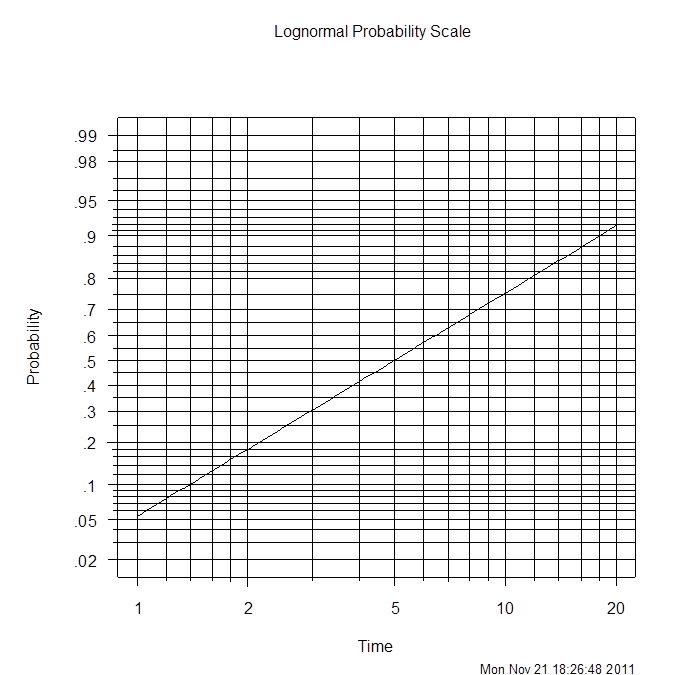
\includegraphics[width = 5in]{lognormal_graph_1.png}
  \caption{Lognormal Probability Plot}
\end{figure}

\subsection{} 
Plot on the paper the LOGNOR\begin{math}(exp(\mu) = 5, \sigma = 1).\end{math}
Explain clearly the process to plot the line.\\

A probability plot linearizes t, some variable, against the CDF of that variable by transforming both variables such that the relationship between the two is linear.  First we start with the quantile function of the CDF.  In the case of the lognormal, this is \(t_p = exp(\mu + \phi_{nor}^{-1} \sigma)\), where \(\phi_{nor}^{-1}\) is the p quantile of the standard normal distribution.  By taking the log of both sides we get \(log(t_p) = \mu + \phi_{nor}^{-1} \sigma\).  This relationship plots as a straight line.  The slope of the line, given that the respective quantile function is the inverse of  \(\phi_{nor}\) is \(1/\sigma\).\\

Therefore the steps use to generate the plot above are as follows:\\
\begin{itemize}
\item Create a sequence of numbers between 0 and 20.\\

\item Log these numbers and calculate respective PDF outputs for the vector based on the normal distribution.  Since the numbers have been logged this is the equivalent to the lognormal distribution.

\item Use the plotprob function in Rsplida, which creates probability paper by plotting each respective axis in log-scale (in this case).

\item Use the lines() function in Rsplida which plots t:time against y:quantiles of time.
\end{itemize}


% Problem 1.b
\begin{figure}
  \centering
  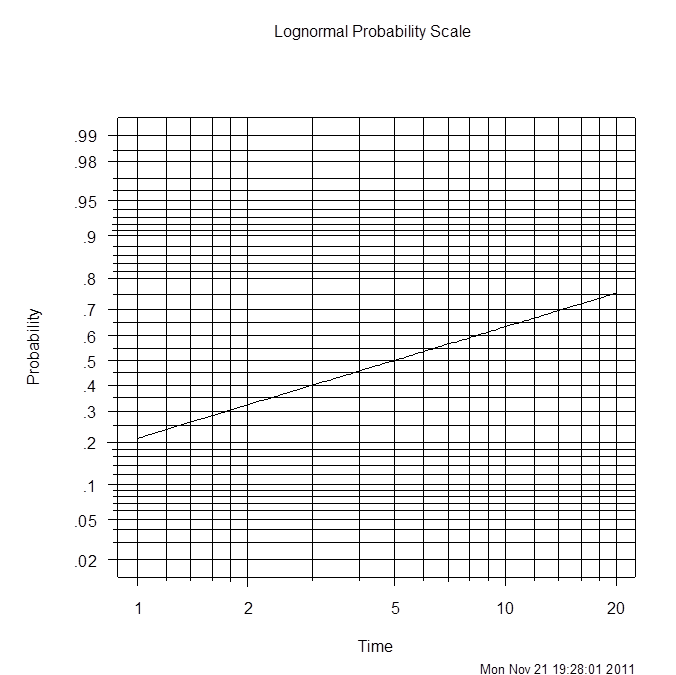
\includegraphics[width = 5in]{lognormal_graph_2.png}
  \caption{Lognormal Probability Plot}
\end{figure}
\FloatBarrier

\subsection{}
Plot on the paper the LOGNOR\begin{math}(exp(\mu) = 5, \sigma = 2).\end{math}
Explain clearly the process to plot the line.\\

A probability plot linearizes t, some variable, against the CDF of that variable by transforming both variables such that the relationship between the two is linear.  First we start with the quantile function of the CDF.  In the case of the lognormal, this is \(t_p = exp(\mu + \phi_{nor}^{-1} \sigma)\), where \(\phi_{nor}^{-1}\) is the p quantile of the standard normal distribution.  By taking the log of both sides we get \(log(t_p) = \mu + \phi_{nor}^{-1} \sigma\).  This relationship plots as a straight line.  The slope of the line, given that the respective quantile function is the inverse of  \(\phi_{nor}\) is \(1/\sigma\).\\

Therefore the steps use to generate the plot above are as follows:\\
\begin{itemize}
\item Create a sequence of numbers between 0 and 20.\\

\item Log these numbers and calculate respective PDF outputs for the vector based on the normal distribution.  Since the numbers have been logged this is the equivalent to the lognormal distribution.

\item Use the plotprob function in Rsplida, which creates probability paper by plotting each respective axis in log-scale (in this case).

\item Use the lines() function in Rsplida which plots t:time against y:quantiles of time.
\end{itemize}


% Problem 2.a
\begin{figure}
  \centering
  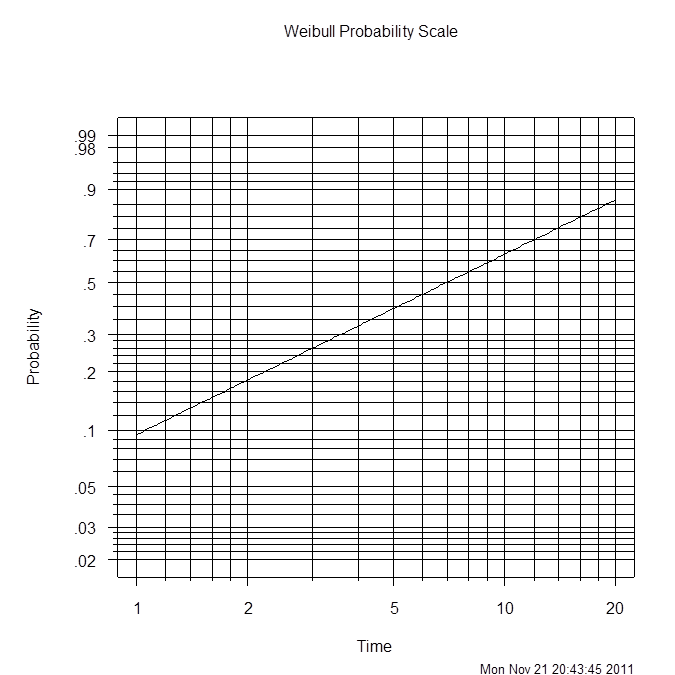
\includegraphics[width = 5in]{weibull_graph_1.png}
  \caption{Weibull Probability Plot}
\end{figure}
\FloatBarrier

\subsection{}
Plot on the paper the WEIB\begin{math}(exp(\eta = 10, \beta = 2).\end{math}
Explain clearly the process to plot the line.\\

A probability plot linearizes t, some variable, against the CDF of that variable by transforming both variables such that the relationship between the two is linear.  First we start with the quantile function of the CDF.  In the case of the Weibull, this is \(t_p = exp(\mu + \phi_{sev}^{-1} \sigma)\), where \(\phi_{sev}^{-1}\) is the p quantile of the standard smallest extreme value distribution.  By taking the log of both sides we get \(log(t_p) = \mu + \phi_{sev}^{-1} \sigma\).  This relationship plots as a straight line.  The slope of the line, given that the respective quantile function is the inverse of  \(\phi_{sev}\) is \(1/\sigma\).\\

Therefore the steps use to generate the plot above are as follows:\\
\begin{itemize}
\item Create a sequence of numbers between 0 and 20.\\

\item Log these numbers and calculate respective PDF outputs for the vector based on the smallest extreme value distribution.  Since the numbers have been logged this is the equivalent to the Weibull distribution.

\item Use the plotprob function in Rsplida, which creates probability paper by plotting each respective axis in log-scale (in this case).

\item Use the lines() function in Rsplida which plots t:time against y:quantiles of time.
\end{itemize}


% Problem 2.b
\begin{figure}
  \centering
  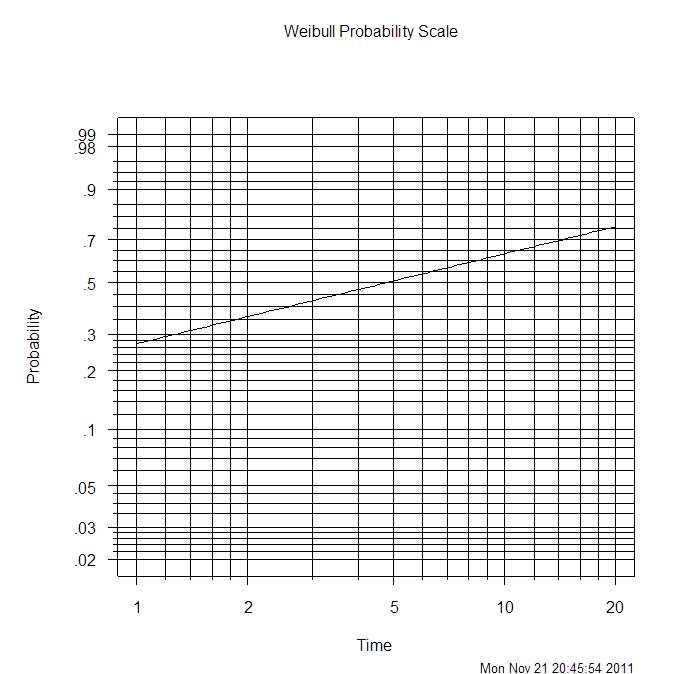
\includegraphics[width = 5in]{weibull_graph_2.png}
  \caption{Weibull Probability Plot}
\end{figure}
\FloatBarrier

\subsection{}
Plot on the paper the WEIB\begin{math}(exp(\eta = 10, \beta = 2).\end{math}
Explain clearly the process to plot the line.\\

A probability plot linearizes t, some variable, against the CDF of that variable by transforming both variables such that the relationship between the two is linear.  First we start with the quantile function of the CDF.  In the case of the Weibull, this is \(t_p = exp(\mu + \phi_{sev}^{-1} \sigma)\), where \(\phi_{sev}^{-1}\) is the p quantile of the standard smallest extreme value distribution.  By taking the log of both sides we get \(log(t_p) = \mu + \phi_{sev}^{-1} \sigma\).  This relationship plots as a straight line.  The slope of the line, given that the respective quantile function is the inverse of  \(\phi_{sev}\) is \(1/\sigma\).\\

Therefore the steps use to generate the plot above are as follows:\\
\begin{itemize}
\item Create a sequence of numbers between 0 and 20.\\

\item Log these numbers and calculate respective PDF outputs for the vector based on the smallest extreme value distribution.  Since the numbers have been logged this is the equivalent to the Weibull distribution.

\item Use the plotprob function in Rsplida, which creates probability paper by plotting each respective axis in log-scale (in this case).

\item Use the lines() function in Rsplida which plots t:time against y:quantiles of time.
\end{itemize}


\end{document}
